\documentclass[t]{beamer}

% --- Theme and Color Setup ---
\usetheme{Madrid}
\definecolor{MyBlue}{RGB}{20, 60, 120}
\usecolortheme[named=MyBlue]{structure}
\setbeamercolor{palette primary}{bg=blue!90!black,fg=white}
\setbeamercolor{palette secondary}{bg=blue!70!black,fg=white}
\setbeamercolor{palette tertiary}{bg=blue!70!black,fg=white}
\setbeamerfont{caption}{size=\footnotesize}

% Packages
\usepackage[utf8]{inputenc}
\usepackage{hyperref}
\usepackage{tikz}
\usepackage{booktabs}
\usepackage{amsmath}
\usepackage{multirow}
\usepackage{colortbl}

% --- Logo on content slides (below title bar) ---
\addtobeamertemplate{frametitle}{}{%
    \begin{tikzpicture}[remember picture,overlay]
        \node[anchor=north east, xshift=-0.2cm, yshift=-0.6cm, inner sep=0pt] at (current page.north east) {
            
\includegraphics[height=0.65cm, keepaspectratio]{logo1.png}
        };
    \end{tikzpicture}%
}

% --- First & Last Page Layout ---
\newcommand{\FirstLastPageLayout}{
    \begin{tikzpicture}[remember picture,overlay]
        \node[anchor=north east, xshift=-0.3cm, yshift=-0.1cm, inner sep=0pt] at (current page.north east) {
            
\includegraphics[height=0.9cm, keepaspectratio]{logo1.png}
        };
        \node[anchor=south west, xshift=0.5cm, yshift=0.5cm] at (current page.south west) {
            \textcolor{MyBlue}{\footnotesize Indian Institute of Technology Patna}
        };
    \end{tikzpicture}
}

% --- Info ---
\title[Topology-Aware Routing]{When Should Language Models Search?\\[0.2em] {\small A Topology-Aware Analysis of Reasoning Strategies}}
\subtitle{M.Tech Thesis Defense}
\author{Md Tanzeel Adam Khan (2411AI67)}
\institute[IIT Patna]{Department of Computer Science and Engineering\\Supervisor: Dr. Asif Ekbal}
\date{June 2026}

\begin{document}

% === SLIDE 1: Title ===
\begin{frame}[plain]
    \FirstLastPageLayout
    \titlepage
\end{frame}

% === SLIDE 2: Research Gap & Aim ===
\begin{frame}{Research Gap \& Aim}

\begin{columns}[T]
\begin{column}{0.55\textwidth}
\textbf{Gap:}
\begin{itemize}\small
    \item CoT = single linear trace; brittle on multi-hop
    \item Search helps \textit{sometimes} --- but when?
    \item Trace-based routers: expensive, misled by fluency
\end{itemize}

\vspace{0.4em}
\textbf{Aim:}
\begin{itemize}\small
    \item Predict CoT vs A* from \textbf{input structure alone}
    \item 13 pre-generation topology features
    \item 8 benchmarks $\times$ 3 scales (QA + Math + Code)
\end{itemize}
\end{column}

\begin{column}{0.42\textwidth}
\centering
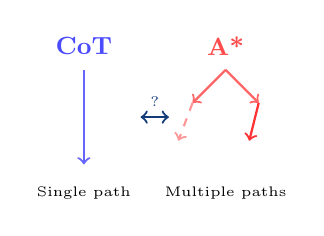
\begin{tikzpicture}[scale=0.6, every node/.style={font=\tiny}]
% CoT
\node[font=\small\bfseries, blue!70] at (0,3) {CoT};
\draw[->, thick, blue!60] (0,2.5) -- (0,2) -- (0,1.5) -- (0,1) -- (0,0.5);
\node[font=\tiny] at (0,-0.1) {Single path};

% A*
\node[font=\small\bfseries, red!70] at (3,3) {A*};
\draw[->, thick, red!60] (3,2.5) -- (2.3,1.8);
\draw[->, thick, red!60] (3,2.5) -- (3.7,1.8);
\draw[->, thick, red!40, dashed] (2.3,1.8) -- (2,1);
\draw[->, thick, red!80] (3.7,1.8) -- (3.5,1);
\node[font=\tiny] at (3,-0.1) {Multiple paths};

% Arrow between
\draw[<->, thick, MyBlue] (1.2,1.5) -- (1.8,1.5) node[midway, above, font=\tiny] {?};
\end{tikzpicture}

\vspace{0.3em}
{\scriptsize\textit{Which one to use? $\rightarrow$ Our router decides}}
\end{column}
\end{columns}

\end{frame}

% === SLIDE 3: Methodology I ===
\begin{frame}{Methodology I: System Overview}

\begin{center}
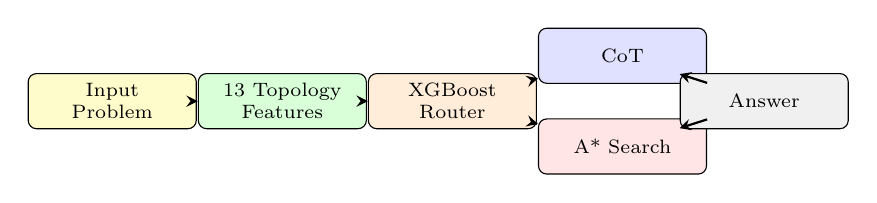
\begin{tikzpicture}[
    scale=0.72, every node/.style={font=\scriptsize},
    block/.style={rectangle, draw, rounded corners=3pt, minimum height=0.7cm, text width=1.9cm, align=center},
    arrow/.style={->, thick, >=stealth}
]
\node[block, fill=yellow!20] (input) at (0,0) {Input\\Problem};
\node[block, fill=green!15] (feat) at (3,0) {13 Topology\\Features};
\node[block, fill=orange!15] (router) at (6,0) {XGBoost\\Router};
\node[block, fill=blue!12] (cot) at (9,0.8) {CoT};
\node[block, fill=red!10] (astar) at (9,-0.8) {A* Search};
\node[block, fill=gray!12] (ans) at (11.5,0) {Answer};

\draw[arrow] (input) -- (feat);
\draw[arrow] (feat) -- (router);
\draw[arrow] (router) -- (cot);
\draw[arrow] (router) -- (astar);
\draw[arrow] (cot) -- (ans);
\draw[arrow] (astar) -- (ans);
\end{tikzpicture}
\end{center}

\vspace{0.2em}
\begin{itemize}\small
    \item \textbf{A* search:} Priority queue over reasoning traces ($f = g + h$), heuristic-guided
    \item \textbf{13 features:} Extracted from input text only (connectives, hops, branching coefficient)
    \item \textbf{No LLM call needed} for routing --- only text analysis
    \item Router trained via 5-fold stratified CV per dataset
\end{itemize}

\end{frame}

% === SLIDE 4: Methodology II ===
\begin{frame}{Methodology II: A* \& Features}

\textbf{A* over Reasoning Traces:}
\begin{itemize}\small
    \item State = partial trace; expand via LLM step generation
    \item $g(n) = d_n + \sum(1{-}c_t)$ \quad $h(n) = \omega_d(H_{\min}{-}d_n) + \omega_c(1{-}E(n))$
    \item Admissible heuristic (proven); budget-limited search
\end{itemize}

\vspace{0.3em}
\textbf{13 Pre-Generation Topology Features:}
\begin{columns}[T]
\begin{column}{0.48\textwidth}
\scriptsize
\begin{enumerate}\setlength{\itemsep}{0pt}
    \item Question length
    \item Context length
    \item Logical connectives
    \item Negation markers
    \item Hop indicators
    \item Comparison words
    \item Question marks
\end{enumerate}
\end{column}
\begin{column}{0.48\textwidth}
\scriptsize
\begin{enumerate}\setlength{\itemsep}{0pt}\setcounter{enumi}{7}
    \item Context sentences
    \item Named entities
    \item Linearity score
    \item Answer options
    \item Depth estimate
    \item Branching complexity
\end{enumerate}
\vspace{0.4em}
\normalsize
$\text{BC} = \frac{\text{ctx\_sents} \times \text{hop}}{\text{q\_len}}$\\[0.2em]
{\tiny Predicts A* advantage: $R^2 = 0.94$}
\end{column}
\end{columns}

\end{frame}

% === SLIDE 5: Results I ===
\begin{frame}{Results I: Main Results}

\begin{table}
\centering
\scriptsize
\setlength{\tabcolsep}{2.5pt}
\begin{tabular}{l|cc|cc|cc}
\toprule
& \multicolumn{2}{c|}{\textbf{8B}} & \multicolumn{2}{c|}{\textbf{0.5B}} & \multicolumn{2}{c}{\textbf{14B}} \\
\textbf{Dataset} & CoT & A* & CoT & A* & CoT & A* \\
\midrule
StrategyQA & 64.5 & \textbf{74.8} & 53.6 & 53.4 & 76.0 & 75.6 \\
LogicQA & \textbf{45.8} & 44.9 & \textbf{24.0} & 20.2 & 57.9 & \textbf{58.1} \\
HotpotQA & 76.8 & \textbf{80.1} & 8.4 & \textbf{30.0} & 60.2 & \textbf{83.3} \\
\midrule
GSM8K & 85.0 & \textbf{86.1} & \textbf{26.8} & 14.5 & 61.6 & \textbf{80.6} \\
MATH & 78.0 & \textbf{79.1} & \textbf{32.8} & 16.2 & 44.0 & \textbf{47.2} \\
\midrule
HumanEval & \textbf{67.5} & 64.4 & \textbf{33.7} & 20.2 & 77.9 & 76.1 \\
MBPP & \textbf{39.8} & 36.8 & \textbf{24.0} & 20.8 & 46.6 & 45.0 \\
CodeContests & 77.4 & \textbf{87.0} & 49.8 & \textbf{68.2} & \textbf{99.6} & 94.4 \\
\bottomrule
\end{tabular}
\end{table}

\vspace{-0.2em}
\begin{itemize}\small
    \item \textbf{Neither dominates.} A* wins on multi-hop/algorithmic; CoT wins on linear tasks
    \item A* \textbf{+19pp} on GSM8K (14B); \textbf{+18.4pp} on CodeContests (0.5B)
    \item Oracle gap up to \textbf{14pp} $\rightarrow$ routing is worthwhile
\end{itemize}

\end{frame}

% === SLIDE 6: Results II ===
\begin{frame}{Results II: Router Comparison}

\begin{columns}[T]
\begin{column}{0.52\textwidth}
\begin{table}
\centering
\scriptsize
\setlength{\tabcolsep}{2pt}
\begin{tabular}{lc}
\toprule
\textbf{Router} & \textbf{Gap\%} \\
\midrule
CoT only & $-$24.6 \\
A* only & $-$10.9 \\
\midrule
Sem.\ Entropy & $-$3.9 \\
LLM-Critic & +9.6 \\
LLM-Judge & +6.6 \\
Random Forest & $-$3.3 \\
\midrule
\rowcolor{green!20}
\textbf{Topology} & \textbf{+40.0} \\
\bottomrule
\end{tabular}
\end{table}
\end{column}

\begin{column}{0.46\textwidth}
\centering
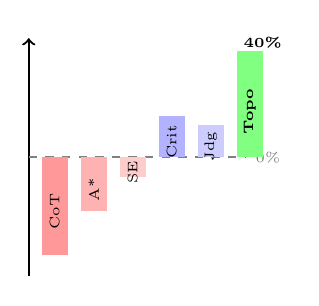
\begin{tikzpicture}[scale=0.55]
\draw[thick, ->] (0,0) -- (0,5.5);
\draw[thick, dashed, gray] (0,2.75) -- (5,2.75) node[right, font=\tiny] {0\%};
\fill[red!40] (0.3,0.5) rectangle (0.9,2.75); \node[font=\tiny,rotate=90] at (0.6,1.5) {CoT};
\fill[red!30] (1.2,1.5) rectangle (1.8,2.75); \node[font=\tiny,rotate=90] at (1.5,2) {A*};
\fill[red!20] (2.1,2.3) rectangle (2.7,2.75); \node[font=\tiny,rotate=90] at (2.4,2.4) {SE};
\fill[blue!30] (3.0,2.75) rectangle (3.6,3.7); \node[font=\tiny,rotate=90] at (3.3,3.1) {Crit};
\fill[blue!20] (3.9,2.75) rectangle (4.5,3.5); \node[font=\tiny,rotate=90] at (4.2,3.0) {Jdg};
\fill[green!50] (4.8,2.75) rectangle (5.4,5.2); \node[font=\tiny,rotate=90] at (5.1,3.8) {\textbf{Topo}};
\node[font=\tiny] at (5.4,5.4) {\textbf{40\%}};
\end{tikzpicture}
\end{column}
\end{columns}

\vspace{0.3em}
\begin{itemize}\small
    \item \textbf{Fluency--Correctness Asymmetry:} 38\% of fluent traces are \textit{wrong}
    \item Post-hoc judges conflate readability with correctness
    \item Topology router sidesteps this --- routes by \textbf{structure alone}
\end{itemize}

\end{frame}

% === SLIDE 7: References ===
\begin{frame}{References}
\tiny
\begin{thebibliography}{10}
\bibitem{wei2022} Wei, J. et al. (2022). Chain-of-thought prompting elicits reasoning in large language models. \textit{NeurIPS}.
\bibitem{yao2024} Yao, S. et al. (2024). Tree of thoughts: Deliberate problem solving with LLMs. \textit{NeurIPS}.
\bibitem{hao2023} Hao, S. et al. (2023). Reasoning with language model is planning with world model. \textit{EMNLP}.
\bibitem{snell2024} Snell, C. et al. (2024). Scaling LLM test-time compute optimally. \textit{arXiv:2408.03314}.
\bibitem{wang2022} Wang, X. et al. (2023). Self-consistency improves chain of thought reasoning. \textit{ICLR}.
\bibitem{hart1968} Hart, P. et al. (1968). A formal basis for heuristic determination of minimum cost paths. \textit{IEEE Trans.}
\bibitem{chen2021} Chen, M. et al. (2021). Evaluating large language models trained on code. \textit{arXiv:2107.03374}.
\bibitem{kossen2024} Kossen, J. et al. (2024). Semantic entropy probes. \textit{arXiv:2406.15927}.
\end{thebibliography}
\end{frame}

% === SLIDE 8: Thank You ===
\begin{frame}[plain]
    \FirstLastPageLayout
    \vfill
    \begin{center}
    {\Huge\bfseries Thank You}
    \end{center}
    \vfill
\end{frame}

\end{document}
